\graphicspath{{2D_QGNIW/figs/}}

The QG-NIW model was derived in \cite{XieVanneste_15}. It has been since further explored and expanded by \cite{WagnerYoung_15, WagnerYoung_16, AsselinYoung_19} and others. Here we will implement the two-dimensional version in \cite{RochaEtAl_18}. 

\section{The nondimensional QG-NIW model}
We have the dimensional QG-NIW model (ignoring dissipation) from \cite[(2.6--8)]{RochaEtAl_18}:
\begin{align}
    &q = \nabla^2\psi + \frac{1}{f}\left[\frac{1}{4}\nabla^2|\phi|^2+\frac{i}{2}J(\phi^*,\phi)\right];\\
    &q_t + J(\psi,q) = 0;\\
    &\phi_t+J(\psi,\phi)+\phi\frac{i}{2}\nabla^2\psi-\frac{i}{2} \frac{N^2}{f m^2} \nabla^2\phi = 0.
\end{align}

We make clear the true parameters dependence of the model by nondimensionalizing the model with:
\begin{align}
    &\phi \sim U_w = \epsilon U_e\\
    &\psi \sim U_e L\\
    &L \sim N/f_0m\\
    &T \sim L/U_e
\end{align}
where
\begin{align}
    \epsilon = {U_w}/{f_0L}\ll 1
\end{align}
indicated we are in the weak wave regime. Then we get (in the notation of \cite{Vallis_96a}):
\begin{align}
    &q = \nabla^2\psi + \frac{1}{f}\{\alpha\}\left[\frac{1}{4}\nabla^2|\phi|^2+\frac{i}{2}J(\phi^*,\phi)\right];\\
    &q_t + J(\psi,q) = 0;\\
    &\phi_t+J(\psi,\phi)+\phi\frac{i}{2}\nabla^2\psi-\frac{i}{2} \frac{N^2}{f m^2} \{\hbar\}\nabla^2\phi = 0
\end{align}
where we have the model depends on only two important nondimensional numbers, the wave amplitude:
\begin{align}
    &\alpha = \frac{U_e}{fL}\epsilon^2 = \text{Ro}\;\epsilon^2,
\end{align}
and the wave dispersivity:
\begin{align}
    &\hbar = \frac{N^2}{fm^2}\frac{1}{LU_e} = \frac{1}{\text{Ro}}\frac{N^2}{f^2 m^2 L^2}.
\end{align}
Note that Rossby number and the small parameter $\epsilon$ does not appear explicitly in the model. We only assume that they are small. Instead, their ratio appear as the wave amplitude $\alpha$. The distinguished limit assumptions in \cite{XieVanneste_15, WagnerYoung_15, WagnerYoung_16} is $\alpha = 1$. However, in \cite{RochaEtAl_18} it is allowed to vary in the $O(1)$ range.

\subsection{Separating the real and imaginary fields}

\section{The Lamb–Chaplygin dipole simulation}

\section{2D turbulence modified by NIW}
\subsection{The parameters}
We use the set-up of \cite[Tabel 4 \& \S 4.2]{RochaEtAl_18}. We pick the nondimensional parameters
\begin{align}
    \alpha = 0.1 \qdt{and} \hbar = 1.
\end{align}
Note that since we have the energy containing scale nondimensionalized to be 1, we have $k_e = 2\pi$ and the domain size to be 10. The $k_e$ value is worth noting when comparing to the results of \cite{RochaEtAl_18}.

\subsection{The balanced flow generation}
We run a 2D Euler simulation to generate the background mean flow using the code in Chapter \ref{chap:2DEuler}. We start the energy near $k_e$ and pick the roughly correct amplitude so that the resulting field matches the amplitude of the \cite{RochaEtAl_18} paper. We let the system evolve and Figure \ref{fig:PVbalanced} the resulting balanced flow. It looks similar to Figure 5(a) of \cite{RochaEtAl_18}. 
\begin{figure}[H]
    \centering
    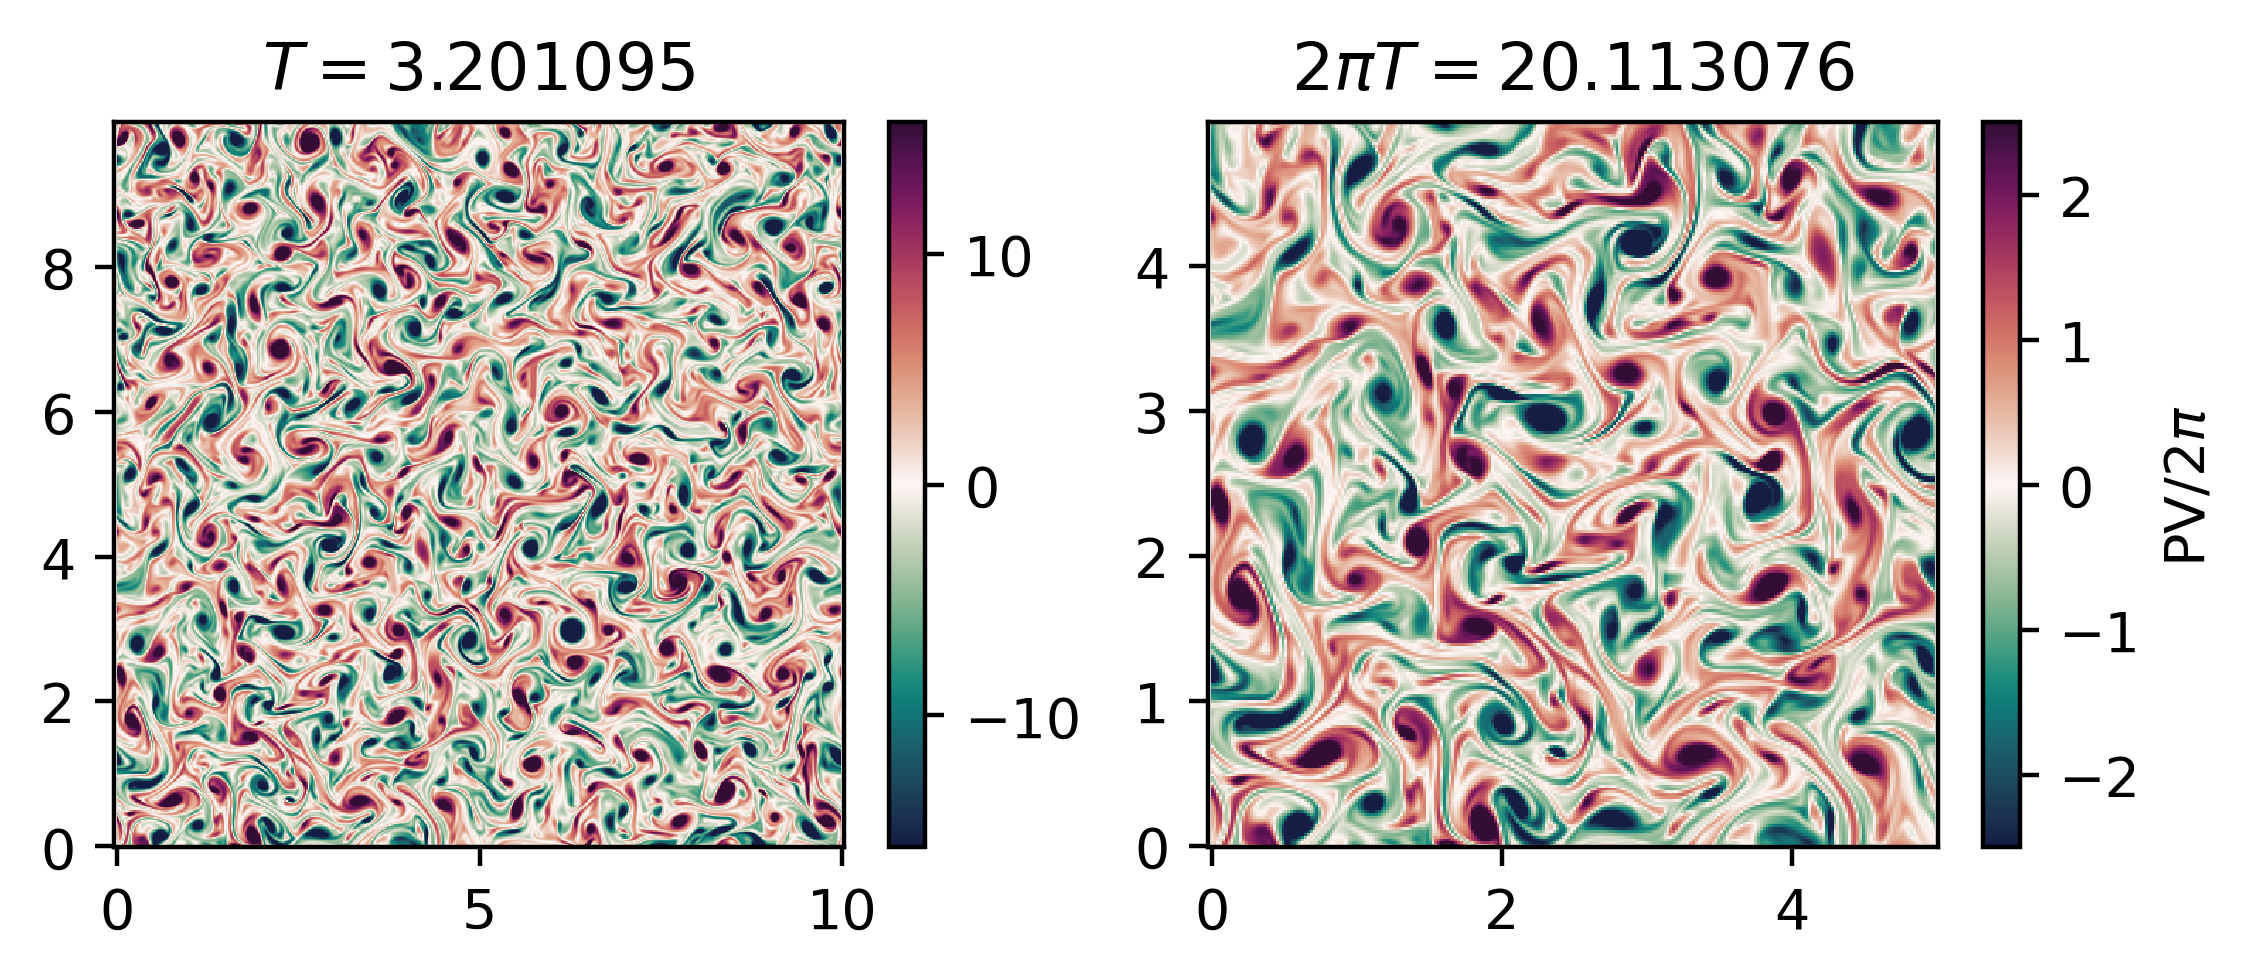
\includegraphics{PVbalanced}
    \caption{Left: the entire PV field. Right: a zoomed in picture of $(1/2)^2$ of the domain, with time and PV scaled so that to match the numbers of \cite{RochaEtAl_18}.}
    \label{fig:PVbalanced}
\end{figure}

\subsection{QG-NIW Simulation}
We simulate the QG-NIW model by adding in a wave field of
\begin{align}
    \phi = \frac{1}{\sqrt{2}}(1+i)
\end{align}
on top of the above PV field. Figure \ref{fig:QGNIW_t1} shows the result. Compare this with Figure 5 of \cite{RochaEtAl_18}, the balanced field looks similar, the action density is weaker (has less variance). We are running a $512^2$ simulation instead of $1024^2$, but this should not create that much of a difference. 
\begin{figure}[H]
    \centering
    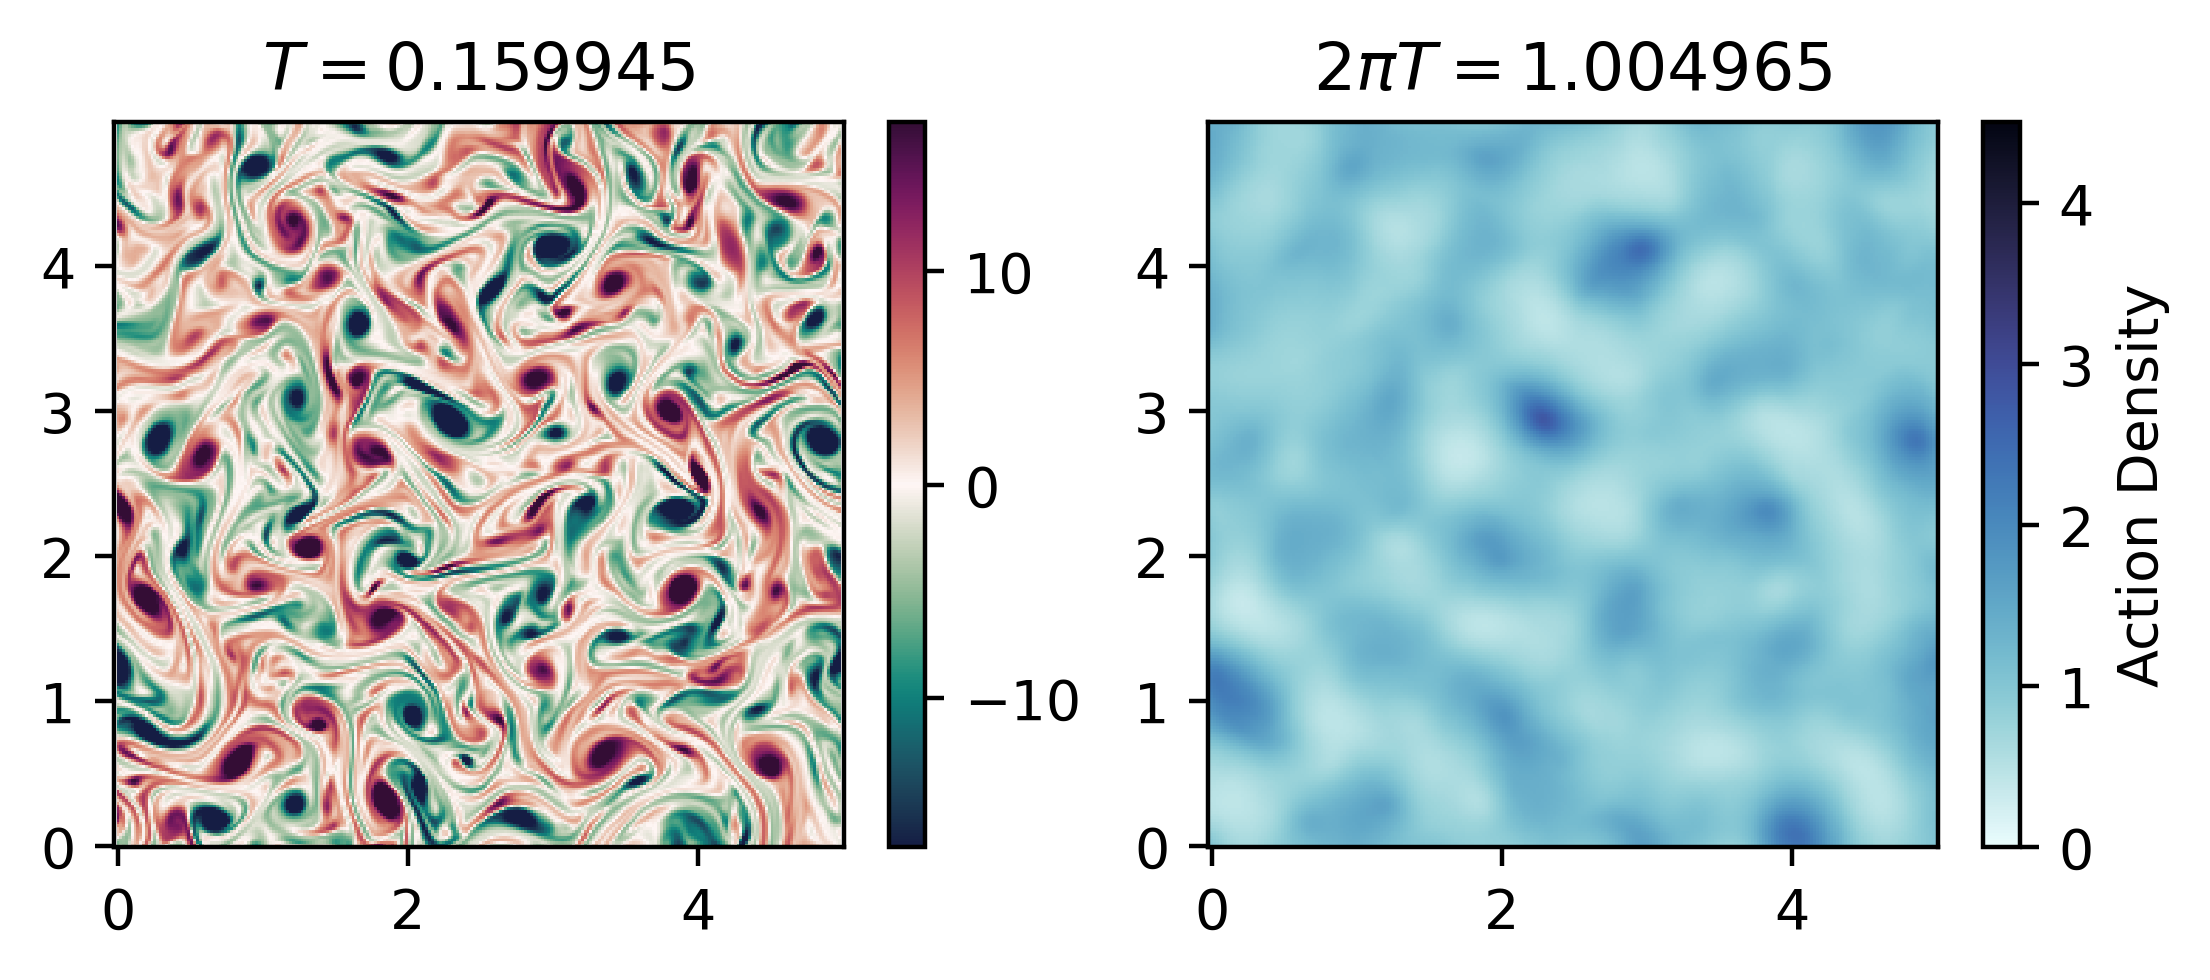
\includegraphics{QGNIW_t1}
    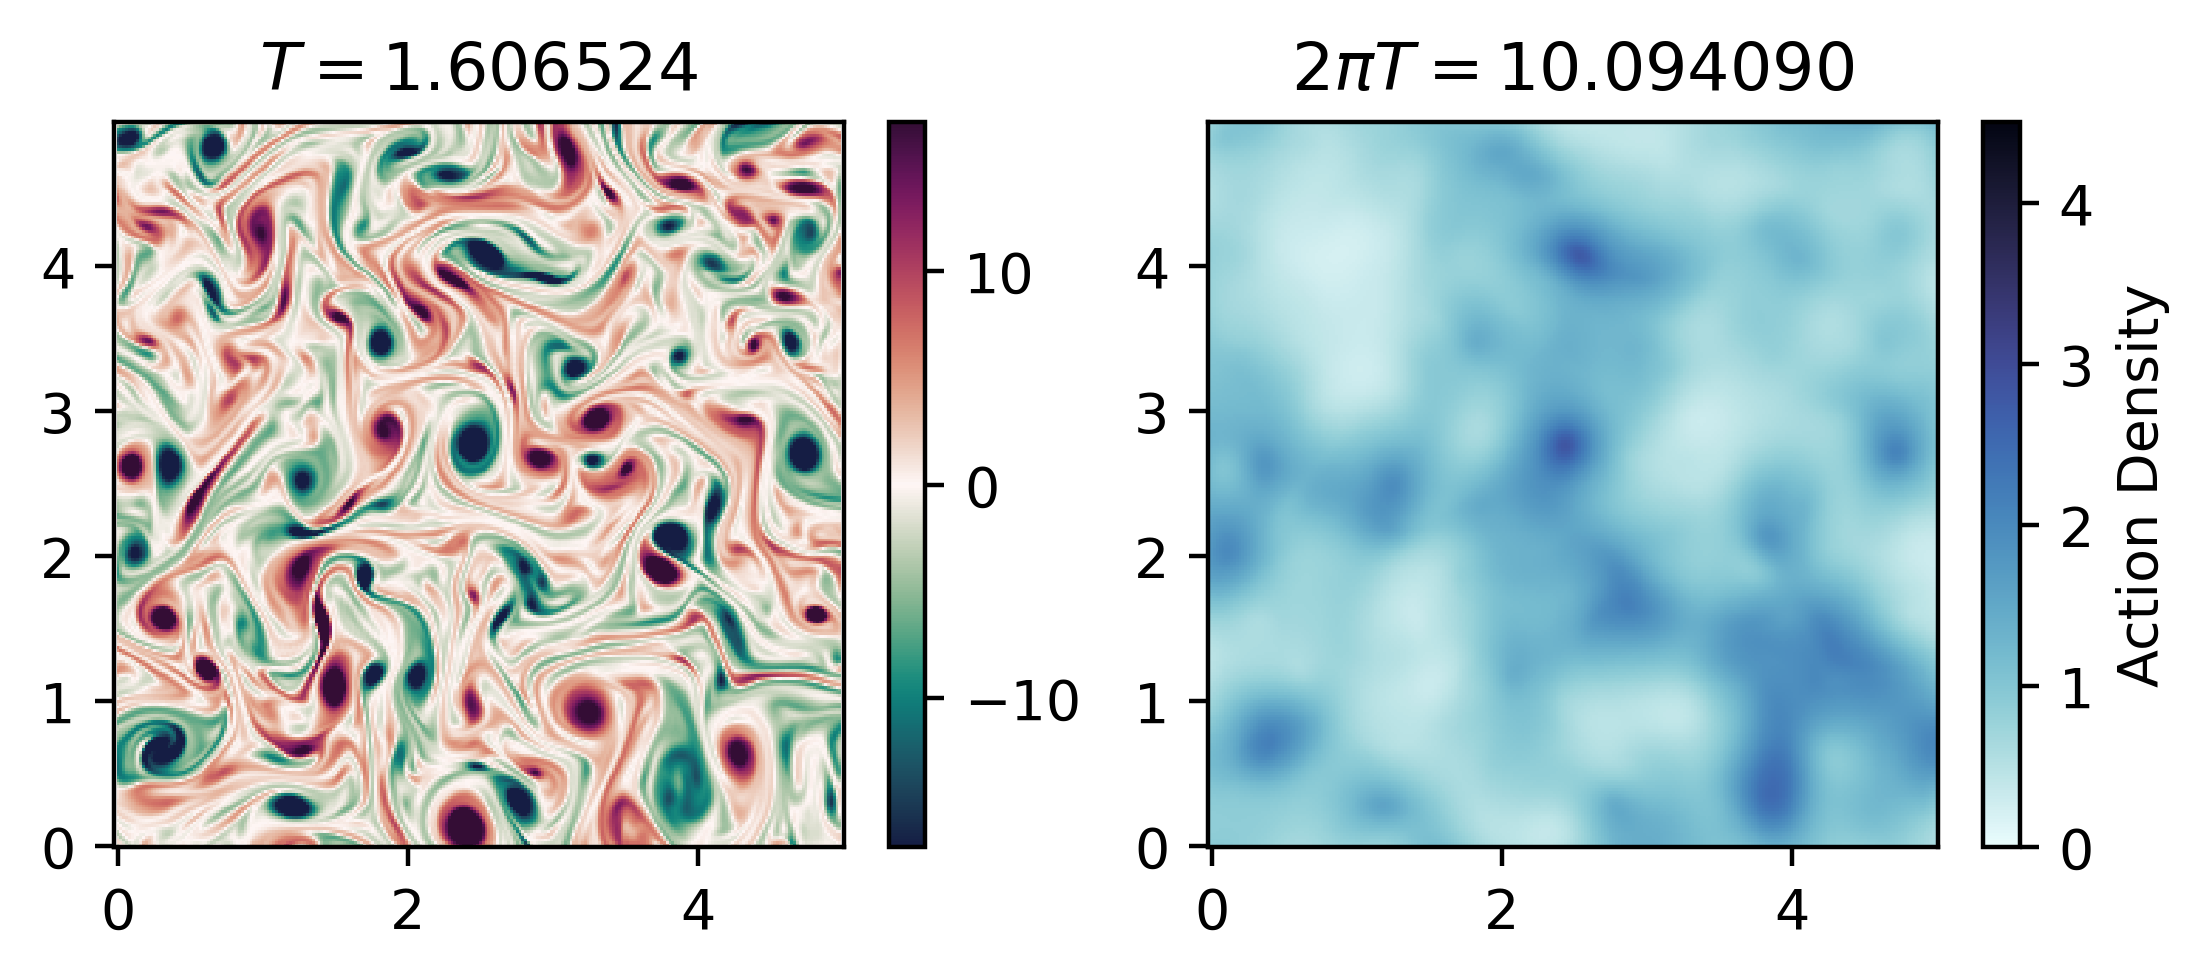
\includegraphics{QGNIW_t10}
    \caption{}
    \label{fig:QGNIW_t1}
\end{figure}

We also track the kinetic energy, potential energy, and action of the simulation. KE get converted into PE, and total energy and action are decreasing slowly. In particular we have the two energies (\cite[3.2]{RochaEtAl_18}):
\begin{align}
    &\mcal{K} = \frac{1}{2}|\nabla\psi|^2;\\
    &\mcal{P} = \frac{1}{4}\frac{N^2}{f^2m^2} |\nabla\phi|^2.
\end{align}
After the nondimensionalization, we have the total energy formula
\begin{align}
    \mcal{P} = \frac{1}{2}|\nabla\psi|^2+\{\alpha\hbar\}\frac{1}{4}\frac{N^2}{f^2m^2} |\nabla\phi|^2.
\end{align}
Note the introduction of the nondimensional numbers in the formula. They need to be accounted for in order for the total energy formula to be correct. 

\subsection{The code}
The code (no data) is in \verb|/scratch/projects/shaferlab/ryan/QGNIW_UNet|. However, right now we cannot run the \verb|QGNIW.py| on Greene because it uses a new Dedalus feature. I am asking Shenglong how to update the Singularity. 

The code is also on Github. I have send you invitations to the repo.



\cite{Conn_2023}.